%%%%%%%%%%%%%%%%%%%%%%%%%%%%%%%%%%%%%%%%%%%%%%%%%%%%%%%%%%%%%%%%%%%%%%%%%%
% SwitchOnBehaviorAndSwitchOffBehaviorOfUI
%%%%%%%%%%%%%%%%%%%%%%%%%%%%%%%%%%%%%%%%%%%%%%%%%%%%%%%%%%%%%%%%%%%%%%%%%%

\begin{figure}[htb]
    \centering
    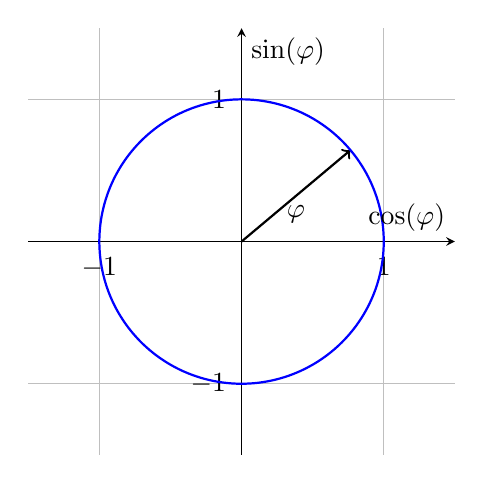
\begin{tikzpicture}
        \begin{axis}[
            axis lines=middle, % Achsen wie im Koordinatensystem
            xlabel={$\cos(\varphi)$},
            ylabel={$\sin(\varphi)$},
            width=7cm, height=7cm,
            grid=both,
            major grid style={line width=.2pt,draw=gray!50},
            minor grid style={line width=.1pt,draw=gray!20},
            xmin=-1.5, xmax=1.5,
            ymin=-1.5, ymax=1.5,
        %    xtick={-1, -0.5, 0, 0.5, 1},
           % ytick={-1, -0.5, 0, 0.5, 1},
        ]
        \draw[thick, ->] (0,0) -- ({cos(40)}, {sin(40)}) node[above right] {};
        \node at ({0.5*cos(40)}, {0.5*sin(40)}) [below] {$\varphi$};
        
        \addplot[
            domain=0:360, % 360° für den ganzen Kreis
            samples=200,  % Anzahl der Punkte
            thick,
            color=blue,
        ]
        ({cos(x)}, {sin(x)}); % Kreisparameter (cos, sin)
    
        \end{axis}
    \end{tikzpicture}
    
    \hspace{1cm} % Abstand zwischen den beiden Diagrammen

    \begin{tikzpicture}
    % Achsen
    \draw[->, thick] (-2,0) -- (2,0) node[right] {$(x)$};
    \draw[->, thick] (0,-2) -- (0,2) node[above] {$(y)$};

    % Punkte auf den Achsen
    \foreach \x in {-2,2} {
        \draw[thick] (\x,0) node[below] {\x} -- (\x,0.2);
    }
    \foreach \y in {-1,1} {
        \draw[thick] (0,\y) -- (0.2,\y) node[right] {\y};
    }

    % Werte cos(k*pi/2)
    \node at (1.5,1.5) {$\cos\left(k \frac{\pi}{2}\right)$};
    \node[below right] at (0.1,0) {1,5,9,...};
    \end{tikzpicture}
    \caption{Switch-on behavior and switch-off behavior of $i_{\mathrm{C}}(t)$.}
    \label{fig:Switch-on behavior and switch-off behavior of}

    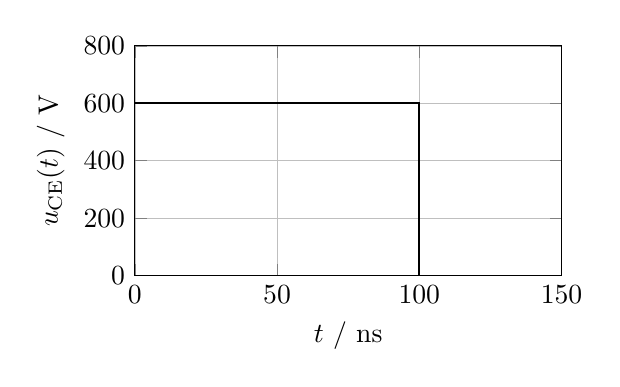
\begin{tikzpicture}
    \begin{axis}[
        width=7cm, height=4.5cm,
        grid=both,
        major grid style={line width=.2pt,draw=gray!50},
        minor grid style={line width=.1pt,draw=gray!20},
        xlabel={$t$ / ns},
        ylabel={$u_{\mathrm{CE}}(t)$ / V},
        xmin=0, xmax=150,
        ymin=0, ymax=800,
        xtick={0, 50, 100, 150},
        ytick={0,200, 400, 600, 800},
        ]
        % Einschaltverhalten graph
        \addplot[
            thick,
            mark=none,
            color=black,
        ] coordinates {
            (0,600) (100, 600) (100, 0)
        };
    \end{axis}
    \end{tikzpicture}
    \hspace{1cm} % Abstand zwischen den beiden Diagrammen
    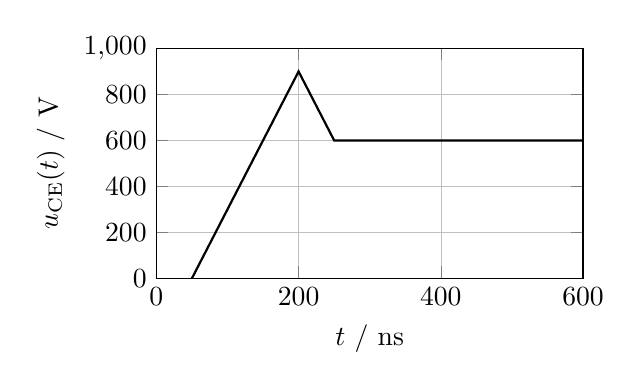
\begin{tikzpicture}
    \begin{axis}[
        width=7cm, height=4.5cm,
        grid=both,
        major grid style={line width=.2pt,draw=gray!50},
        minor grid style={line width=.1pt,draw=gray!20},
        xlabel={$t$ / ns},
        ylabel={$u_{\mathrm{CE}}(t)$ / V},
        xmin=0, xmax=600,
        ymin=0, ymax=1000,
        xtick={0,200, 400, 600},
        ytick={0,200, 400, 600,800, 1000},
        ]
        % Ausschaltverhalten graph
        \addplot[
            thick,
            mark=none,
            color=black,
        ] coordinates {
            (50,0) (200, 900) (250, 600) (600, 600)
        };
    \end{axis}
    \end{tikzpicture}
    \caption{Switch-on behavior and switch-off behavior of $u_{\mathrm{CE}}(t)$.}
    \label{fig:Switch-on behavior and switch-off behavior of voltage}
\end{figure}
